\begin{enumerate}[label=\thesection.\arabic*.,ref=\thesection.\theenumi]
\numberwithin{equation}{enumi}

\item
For the unity feedback system shown in Fig. \ref{fig:ee18btech11049_block_1} , with 
\begin{align}
    G(s) = \frac{K}{s(s+1)(s+4)}
\end{align}
Design a lag-lead
compensator to yield a  $K_{v} = 12$ as well as peak overshoot
of 12\% and peak time of less than or equal to 2 seconds.
\begin{figure}[!ht]
\begin{center}
	\resizebox{\columnwidth}{!}{.\input{./figs/ee18btech11049/ee18btech11049_block_1.tex}}
\end{center}
    \caption{}
    \label{fig:ee18btech11049_block_1}
\end{figure}

\item
\solution

\begin{align}
    K_{v} = \lim_{s \to 0} s G(s) = 12\\
    \implies K = 48
\end{align}
The bode plot for G(s)is as follows : 

\begin{align}
    G(s) = \frac{48}{s(s+1)(s+4)}
\end{align}

\begin{figure}[!h]
    \centering
    \includegraphics[width=\columnwidth]{./figs/ee18btech11049/ee18btech11049_1.eps}
    \caption{G(s) Bode Plot}
    \label{fig:ee18btech11049_1}
\end{figure}

Damping Ratio $\zeta$
\begin{align}
    \zeta = \frac{-\ln\left(\frac{OS\%}{100}\right)}{\sqrt{\pi^2+\left(\ln\left(\frac{OS\%}{100}\right)\right)^2}}
\end{align}
Phase Margin $\phi_{M}$
\begin{align}
    \phi_{M} = \tan^{-1}\left(\frac{2\zeta}{\sqrt{-2\zeta^2 + \sqrt{4\zeta^4 + 1}}}\right)  
\end{align}
closed-loop Bandwidth $\omega_{bw}$
\begin{align}
    \omega_{bw} = \frac{\pi}{T_{p}\sqrt{1-\zeta ^2}}\sqrt{1-2\zeta^2+\sqrt{4\zeta^4 - 4\zeta ^2 + 2}}
\end{align}

The following code computes the above quantities.
\begin{lstlisting}
codes/ee18btech11049/ee18btech11049_1.py
\end{lstlisting}
\begin{align}
    \zeta  =  0.557\\
    \phi_{M} = 56.13\degree\\
     \omega_{bw} = 2.27 \text{ rad/sec }
\end{align}{}



The required phase margin to yield a 12\% OS is 56.13\degree \\
Let us select  $\omega = $1.83 rad/s as the new phase-margin frequency. \\At this frequency, the uncompensated phase is -176 and would require, if we
add a -6 contribution from the lag compensator, a +56 contribution from the
lead compensator.

\begin{align}
    G_{Lead}\brak{s}G_{Lag}\brak{s} = \left(\frac{s+\frac{1}{T_1}}{s+\frac{\gamma}{T_1}}\right)\left(\frac{s+\frac{1}{T_2}}{s+\frac{1}{\gamma T_2}}\right)
\end{align}

Choose the lag compensator 1-decade below, so that its
will have minimal effect at the new phase-margin frequency.
\begin{align}
     \phi_{max,lead} = 56 = \sin^{-1}{\frac{1-\beta}{1+\beta}}
\end{align}
\begin{align}
    \beta = 0.092 
\end{align}
\begin{align}
      \gamma = 10.86 \text{   since  } \gamma = \frac{1}{\beta}
\end{align}
Thus with $\gamma$ = 10.86 
\begin{align}
    G_{Lag}\brak{s} = \left(\frac{s+\frac{1}{T_2}}{s+\frac{1}{\gamma T_2}}\right)=  \frac{s+0.183}{s+0.0168}
\end{align}
\begin{align}
    \omega_{max} = \frac{1}{T_1 \sqrt{\beta}}
\end{align}

Using Values of $\omega_{max}  = 1.83 $ and $\beta = 0.094$
\begin{align}
     G_{Lag}\brak{s} = \left(\frac{s+\frac{1}{T_1}}{s+\frac{\gamma}{T_1}}\right) = \frac{s+0.55}{s+5.69}
\end{align}

The lag-lead Compensated System's open loop transfer function is
\begin{align}
  G_{total}\brak{s} =  \frac{48\brak{s+0.183}\brak{s+0.55}}{s\brak{s+1}\brak{s+4}\brak{s+0.0168}\brak{s+5.69}}
\end{align}
\begin{figure}[!h]
    \centering
    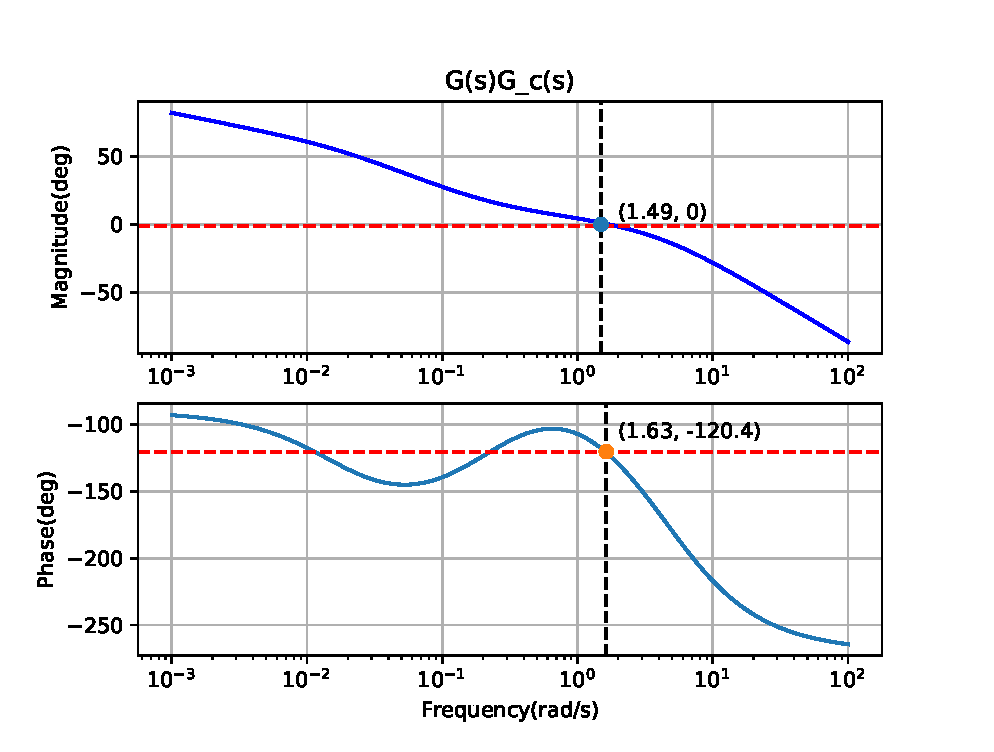
\includegraphics[width=\columnwidth]{./figs/ee18btech11049/ee18btech11049_2.eps}
    \caption{G(s) Compensated Bode Plot}
    \label{fig:ee18btech11049_2}
\end{figure}


\item
\textbf{Verification : }
We could observe the  affect of the lag-lead  compensator from these phase plots.\\

\begin{figure}[!h]
    \centering
    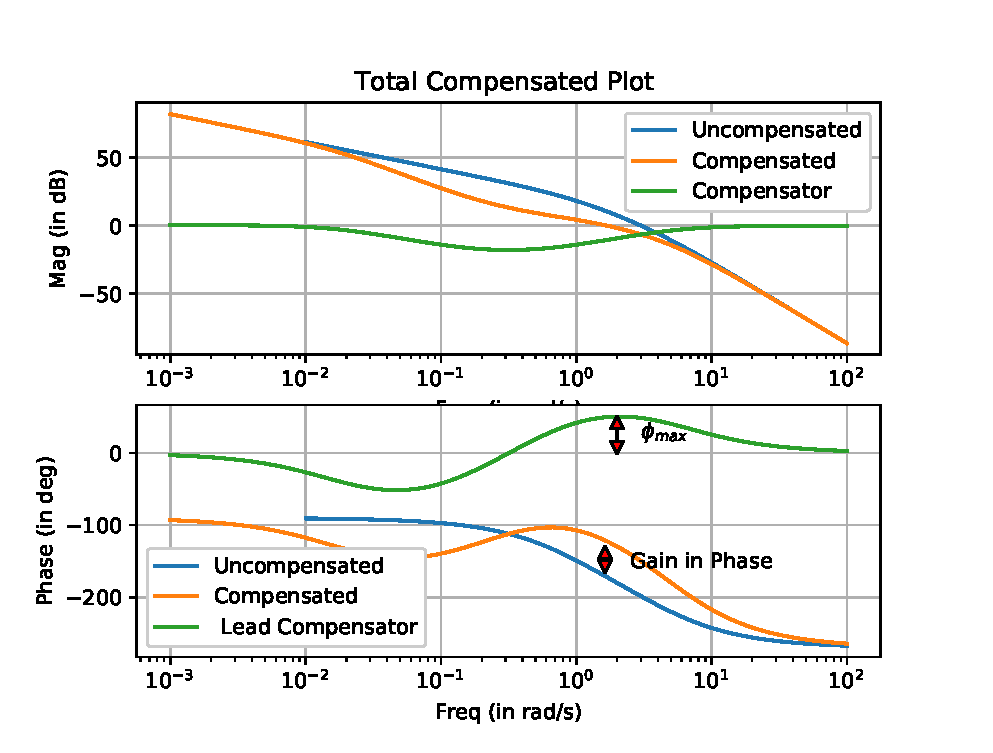
\includegraphics[width=\columnwidth]{./figs/ee18btech11049/ee18btech11049_3.eps}
    \caption{Combined Bode Plots}
    \label{fig:ee18btech11049_3}
\end{figure}






These plots are generated using the below code:
\begin{lstlisting}
codes/ee18btech11049/ee18btech11049_2.py
\end{lstlisting}
\item
\textbf{Result :}
The below is the summary for the designed lead-lead compensator.\\

\begin{table}[!ht]
\centering
\input{./tables/ee18btech11049/ee18btech11049_table_1.tex}
\caption{Comparing the desired and obtained results}
\label{table:ee18btech11049_table_1}
\end{table}








\end{enumerate}
